\documentclass[border=4pt,12pt]{standalone}
% House style for redrawn exam diagrams (diagram-v4: 0.4pt lines, filled -latex arrows, fine dashes; stipple and hatching drawn as real dots/lines (no PDF/SVG patterns, so they render in every browser and at any scale); transparent background). Every figure \input's this.
\usepackage{amsmath,amssymb}
\usepackage{txfonts}
\usepackage{pdfrender,xcolor}
% \halo{text}: label on shading. The shading stops just around each letter's outline (a thin knock-out that follows the
% glyphs, like the papers' typesetting), never a box. Owner: "I don't want a box around the text".
\newcommand{\halo}[1]{\leavevmode\rlap{\pdfrender{TextRenderingMode=2,LineWidth=2.2pt,LineJoinStyle=1,StrokeColor=white,FillColor=white}#1}#1}
\usepackage{tikz,pgfplots}
\pgfplotsset{compat=1.18}
\usetikzlibrary{arrows.meta,calc,angles,quotes,patterns,patterns.meta,intersections,positioning,decorations.markings,shapes.geometric}
% Stipple and hatching are drawn as actual dots / lines clipped to the region (path picture), NOT as pattern fills:
% SVG <pattern> fills vanish or blur when browsers scale the image, so the owner could not see the shading.
% Each dot is a 0.72pt square (keeps SVGs small; reads as a dot at print size). Dots sit on one global staggered grid, so neighbouring regions line up.
\makeatletter
\newdimen\ex@x \newdimen\ex@y \newdimen\ex@xa \newdimen\ex@ya \newdimen\ex@xb \newdimen\ex@yb \newcount\ex@row
\def\exam@stipplecolor{black!75}\def\exam@dotr{0.42pt}\def\exam@dotgap{2.5}
\def\ex@rowdots{\ifdim\ex@x<\ex@xb \pgfpathrectangle{\pgfqpoint{\dimexpr\ex@x-0.36pt\relax}{\dimexpr\ex@y-0.36pt\relax}}{\pgfqpoint{0.72pt}{0.72pt}}\advance\ex@x by \exam@dotgap pt\relax\expandafter\ex@rowdots\fi}
\def\exam@stipple{%
  \pgftransformreset% dots are sized in real points even inside scaled pictures
  \pgfpointanchor{path picture bounding box}{south west}\ex@xa=\pgf@x \ex@ya=\pgf@y
  \pgfpointanchor{path picture bounding box}{north east}\ex@xb=\pgf@x \ex@yb=\pgf@y
  \pgfsetfillcolor{\exam@stipplecolor}\pgfmathsetmacro\ex@h{\exam@dotgap/2}%
  \pgfmathtruncatemacro\ex@r{floor(\ex@ya/\ex@h)-1}\ex@row=\ex@r\relax
  \ex@y=\ex@r\dimexpr\ex@h pt\relax
  \loop\ifdim\ex@y<\ex@yb
    \pgfmathtruncatemacro\ex@c{floor(\ex@xa/\exam@dotgap)-1}\ex@x=\ex@c\dimexpr\exam@dotgap pt\relax
    \ifodd\ex@row \advance\ex@x by \ex@h pt\fi
    \ex@rowdots
    \advance\ex@y by \ex@h pt \advance\ex@row by 1
    \ifnum\numexpr\ex@row-(\ex@row/4)*4\relax=0 \pgfusepath{fill}\fi% flush every 4 rows: bounded TeX memory, few clip copies in the SVG
  \repeat\pgfusepath{fill}}
\newdimen\ex@d
\def\exam@hatch#1{% #1 = 1 for /, -1 for \ ; lines 45 degrees, 3pt apart
  \pgftransformreset
  \pgfpointanchor{path picture bounding box}{south west}\ex@xa=\pgf@x \ex@ya=\pgf@y
  \pgfpointanchor{path picture bounding box}{north east}\ex@xb=\pgf@x \ex@yb=\pgf@y
  \ex@d=\dimexpr\ex@yb-\ex@ya\relax \ex@x=\dimexpr\ex@xa-\ex@d\relax
  \loop\ifdim\ex@x<\ex@xb
    \ifnum#1>0 \pgfpathmoveto{\pgfqpoint{\ex@x}{\ex@ya}}\pgfpathlineto{\pgfqpoint{\dimexpr\ex@x+\ex@d\relax}{\ex@yb}}%
    \else \pgfpathmoveto{\pgfqpoint{\ex@x}{\ex@yb}}\pgfpathlineto{\pgfqpoint{\dimexpr\ex@x+\ex@d\relax}{\ex@ya}}\fi
    \advance\ex@x by 4.24pt
  \repeat
  \pgfsetlinewidth{0.4pt}\pgfsetstrokecolor{black}\pgfusepath{stroke}}
\def\examstipple{\exam@stipple}\def\examhatch{\exam@hatch}\def\examsetstipplecolor#1{\def\exam@stipplecolor{#1}}\def\examsetdotgap#1{\def\exam@dotgap{#1}}
\makeatother
% (legacy pattern kept for old files)
% staggered stipple like the NESA papers' dotted shading
\pgfdeclarepatternformonly{exam stipple}{\pgfpointorigin}{\pgfqpoint{2.2pt}{2.2pt}}{\pgfqpoint{2.2pt}{2.2pt}}{%
  \pgfpathcircle{\pgfqpoint{0.55pt}{0.55pt}}{0.42pt}\pgfpathcircle{\pgfqpoint{1.65pt}{1.65pt}}{0.42pt}\pgfusepath{fill}}
\tikzset{
  every picture/.style={line width=0.6pt, >={Latex[length=2mm,width=1.3mm]}},
  curve/.style={line width=0.6pt},
  open arrow/.style={-{Latex[length=2mm,width=1.3mm]}},  % owner: filled -latex heads everywhere, no open chevrons
  aux/.style={dash pattern=on 2pt off 1.5pt, line width=0.6pt},
  shade/.code={\def\exA{#1}\def\exB{none}\ifx\exA\exB\else\pgfkeysalso{fill=black!18}\fi},
  shade/.default=on,
  shade dots/.style={fill=none, path picture={\examstipple}},
  stipple color/.code={\examsetstipplecolor{#1}},
  stipple gap/.code={\examsetdotgap{#1}},
  shade dense dots/.style={fill=none, stipple gap=1.6, path picture={\examstipple}},
  shade hatch/.style={fill=none, path picture={\examhatch{1}}},
  shade hatch reverse/.style={fill=none, path picture={\examhatch{-1}}},
  shade solid/.style={fill=black},
  pt/.style={circle, fill, inner sep=1.1pt},
  open pt/.style={circle, draw, fill=white, inner sep=1.1pt},
}
\pgfplotsset{
  exam axes/.style={axis lines=middle, axis line style={->}, xlabel={$x$}, ylabel={$y$},
    xlabel style={anchor=west}, ylabel style={anchor=south}, tick label style={font=\small},
    every axis plot/.append style={line width=0.6pt, black}, samples=200, clip=false,
    enlargelimits=false, axis on top},
}

\begin{document}
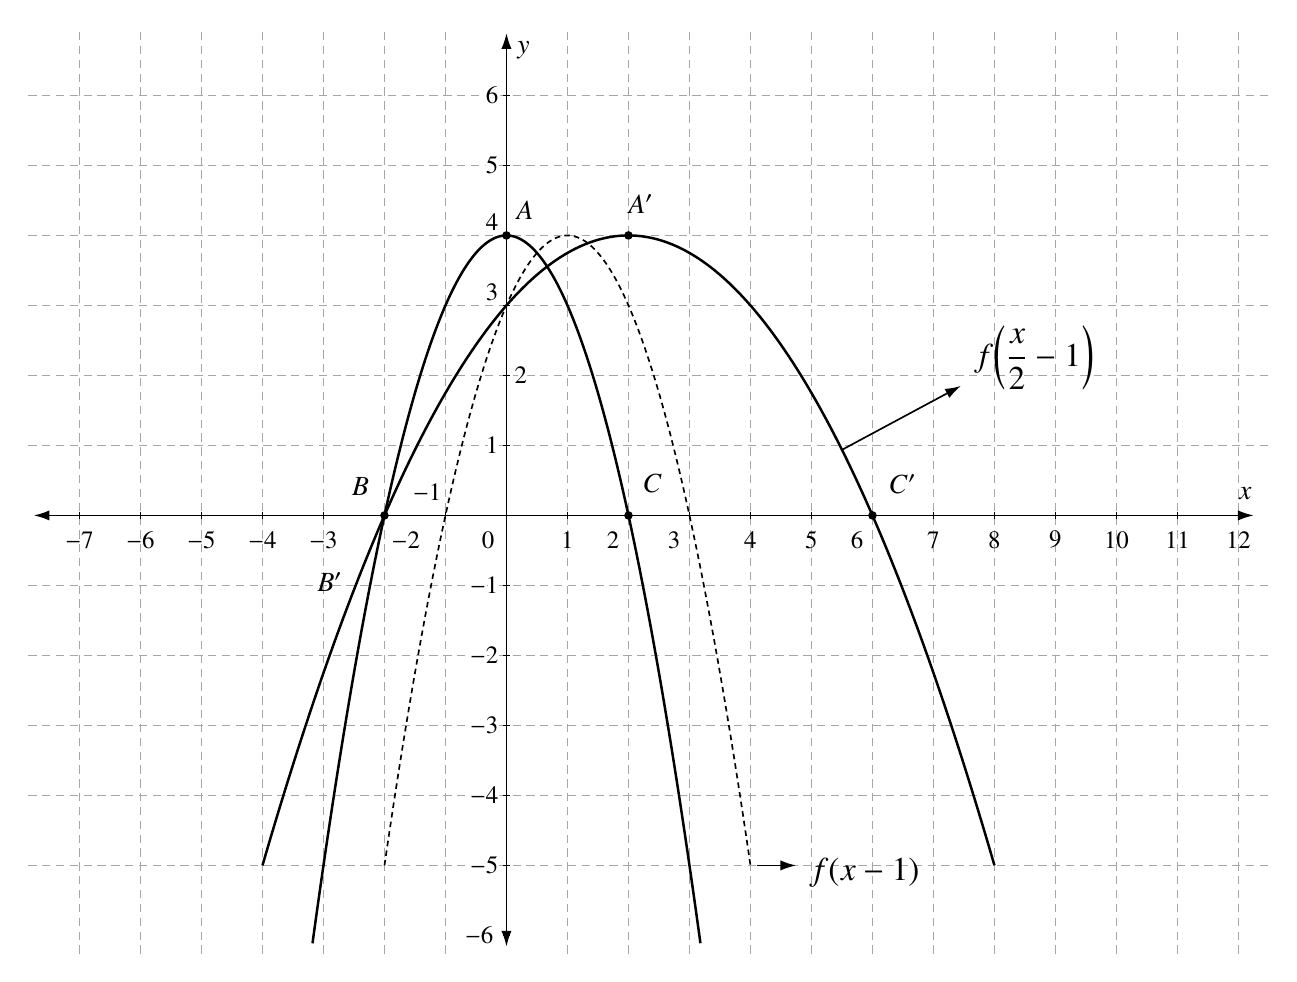
\begin{tikzpicture}[x=0.7747cm,y=0.889cm,font=\small]
\tikzset{gridl/.style={black!35,line width=0.4pt,dash pattern=on 3pt off 2pt}}
\foreach \i in {-7,...,-1,1,2,...,12} \draw[gridl] (\i,-6.26) -- (\i,6.96);
\draw (-0.06,-6) -- (0.06,-6); \node[anchor=east,inner sep=0pt] at (-0.2,-6) {\halo{$-6$}}; % clear of the axis arrowhead
\foreach \j in {-5,...,-1,1,2,...,6} \draw[gridl] (-7.84,\j) -- (12.49,\j);
\draw[<->] (-7.75,0) -- (12.25,0);
\draw[<->] (0,-6.16) -- (0,6.89);
\foreach \i in {-7,...,-3,1,4,5,7,8,...,12} {\draw (\i,0.05) -- (\i,-0.05); \node at (\i,-0.35) {$\i$};}
\foreach \i/\p in {-2/-1.65,2/1.75,3/2.75,6/5.75} {\draw (\i,0.05) -- (\i,-0.05); \node at (\p,-0.35) {$\i$};}
\draw (-1,0.05) -- (-1,-0.05); \node at (-1.3,0.33) {$-1$};
% 25 Nov label-overlap fix (owner 25 Nov: "fix the misdrawn overlaps in the current imports"): y-axis numbers left of the axis, clear of
% it and the ticks, \halo over the grid lines;
% all three curves cross the axis at (0,3) and f(x-1) runs just left of it at y=2, so (DIAGRAM_SPEC 21 Nov): "3" and "4" just above
% their ticks on the left, "2" at the mirror position right of the axis.
\draw (-0.06,-6) -- (0.06,-6); \node[anchor=east,inner sep=0pt] at (-0.2,-6) {\halo{$-6$}}; % clear of the axis arrowhead
\foreach \j in {-5,...,-1,1,5,6} {\draw (-0.06,\j) -- (0.06,\j); \node[anchor=east,inner sep=0pt] at (-0.12,\j) {\halo{$\j$}};}
\draw (-0.06,2) -- (0.06,2); \node[anchor=west,inner sep=0pt] at (0.12,2) {\halo{$2$}};
\draw (-0.06,3) -- (0.06,3); \node[anchor=south east,inner sep=0pt] at (-0.12,3.06) {\halo{$3$}};
\draw (-0.06,4) -- (0.06,4); \node[anchor=south east,inner sep=0pt] at (-0.12,4.06) {\halo{$4$}};
\node at (-0.3,-0.35) {$0$};
\node[font=\normalsize] at (12.1,0.32) {$x$};
\node[font=\normalsize] at (0.28,6.65) {$y$};
% y = f(x)
\draw[line width=0.9pt] plot[domain=-3.18:3.18,smooth,samples=90] (\x,{4-\x*\x});
% y = f(x-1), intermediate step
\draw[aux] plot[domain=-2:4,smooth,samples=90] (\x,{4-(\x-1)*(\x-1)});
% y = f(x/2 - 1)
\draw[line width=0.9pt] plot[domain=-4:8,smooth,samples=90] (\x,{4-(\x/2-1)*(\x/2-1)});
\foreach \q in {(0,4),(-2,0),(2,0),(2,4),(6,0)} \node[pt] at \q {};
\node[font=\normalsize] at (0.3,4.35) {$A$};
\node[font=\normalsize] at (-2.4,0.42) {$B$};
\node[font=\normalsize] at (2.4,0.45) {$C$};
\node[font=\normalsize] at (2.2,4.45) {$A'$};
\node[font=\normalsize] at (-2.9,-0.95) {$B'$};
\node[font=\normalsize] at (6.5,0.45) {$C'$};
\draw[->] (5.5,0.9375) -- (7.45,1.85);
\node[font=\large,anchor=west] at (7.5,2.25) {$f\!\left(\dfrac{x}{2}-1\right)$};
\draw[->] (4.1,-5) -- (4.75,-5);
\node[font=\large,anchor=west] at (4.8,-5.1) {$f(x-1)$};
\end{tikzpicture}
\end{document}